\appendix
\chapter{Additional Experiments}

% \section{\gpp usage}
% \label{appendix:corpus-phonemizer-usage}

% \lstset{basicstyle=\small\ttfamily}
% \begin{lstlisting}[float=tp, breaklines=true,caption={An extract taken from the help menu of \gpp, displaying the tool's usage.}]

% usage: corpus_phonemizer.py [-h] [-k] [-v] [-u] [-i INPUT_FILE]
%        [-o OUTPUT_FILE] {epitran,phonemizer,pingyam,pinyin_to_ipa} language

% Phonemize utterances using a specified backend and language.

% positional arguments:
%   {epitran,phonemizer,pingyam,pinyin_to_ipa}
%                                         The backend to use for phonemization.
%   language                              The language to phonemize.

% options:
%   -h, --help                            show this help message and exit
%   -k, --keep-word-boundaries            Keep word boundaries in the output.
%   -v, --verbose                         Print debug information.
%   -u, --uncorrected                     Use the wrapper's output without
%                                         applying a folding dictionary to correct
%                                         the phoneme sets.
%   -i INPUT_FILE, --input-file INPUT_FILE
%                                         Input file containing utterances (one
%                                         per line). If not specified, reads from
%                                         stdin.
%   -o OUTPUT_FILE, --output-file OUTPUT_FILE
%                                         Output file for phonemized utterances.
%                                         If not specified, writes to stdout.

% Example usage:
%   python corpus_phonemizer.py epitran --language eng-Latn --keep-word-boundaries --verbose < input.txt > output.txt
% \end{lstlisting}

% \section{Corpus Phonemizer Folding Dictionaries}
% \label{appendix:folding-dictionaries}

\section{Average Information Density of Transcribed Child-Directed Speech Increases with Age Cross-Lingually}\label{app:parentese}

\Zeb{I worry that this experiment is too half-baked even for the appendix. I'm thinking I should either remove it, or try to expand it a bit and use it as analysis of \ipachildes in \cref{chapter:resources}.}

The phonemic representation of the utterances in \ipachildes open up new avenues for exploring the phonotactic properties of languages and the information-theoretic properties of child-directed speech. %Previous research in these areas have had to base their calculations on word types \citep{piantadosi2011word, dautriche2017words, pimentel2020phonotactic} or orthographic text \citep{mahowald2013info, dautriche2017wordform, futrell2020lossy}, often citing a lack of phonemic data as a limiting factor. %For instance, \citet{piantadosi2011word} show a strong correlation between information and word length across 10 languages using orthographic data, stating that orthographic word length is correlated with phonetic length, but this may not be the case for certain languages. 

%This representation may be useful when comparing languages that have different levels of orthographic transparency (the correspondence between how words are written and how words are pronounced). 

\begin{figure}
    \centering
    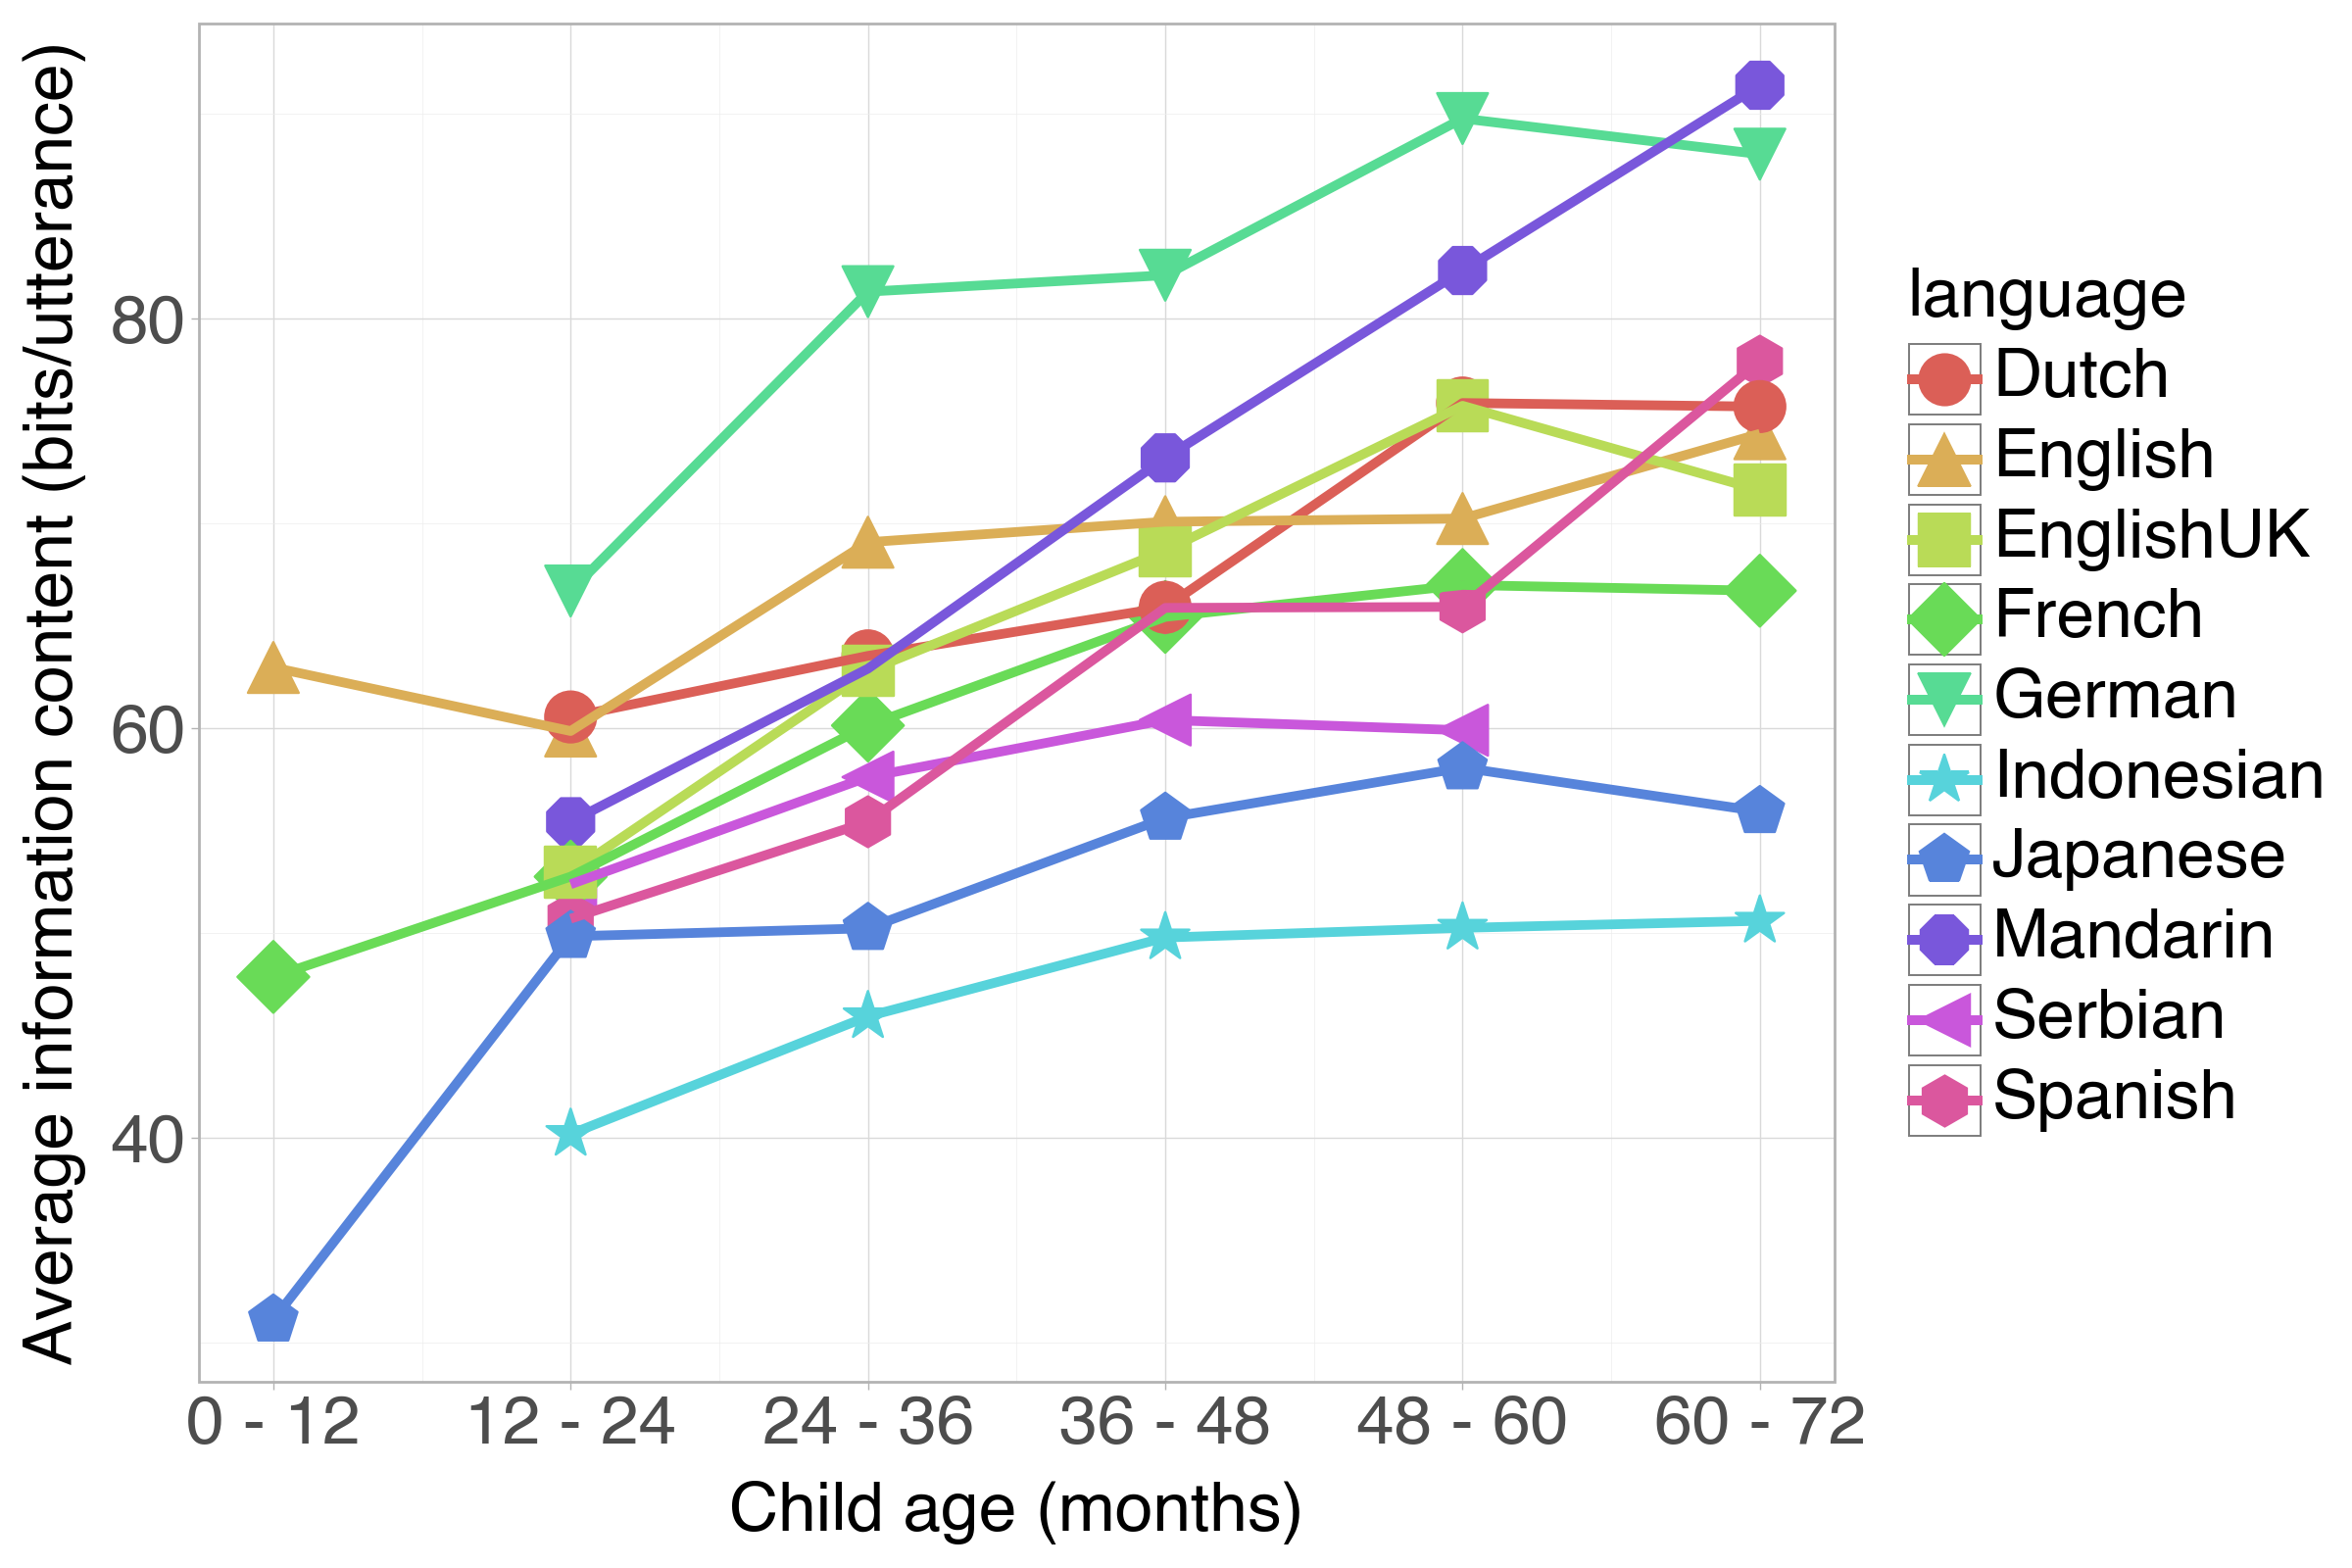
\includegraphics[width=0.99\linewidth]{13Resources/information-trends.png}
    \caption{Average information of child-directed utterances in CHILDES}
    \label{fig:13-information-trends}
\end{figure}

Here, one information-theoretic experiment is demonstrated, comparing the average information content of child-directed utterances to the age of the child being spoken to (this information is also available in CHILDES and is preserved in \ipachildes). Child ages are grouped in years (0-12 months, 12-24 months, etc.) and calculate the average information content of a sample of child-directed utterances using a unigram language model. The information $I_U$ of each utterance consisting of a sequence of phonemes $p_1,p_2,\ldots,p_n$ is given by

$$I_U = -\sum_{i=0}^{n}{log_2P(p_i)},$$

where $P(p_i)$ is the probability of phoneme $p_i$ given by its frequency in the data. The average information of utterances in each age category for the largest 10 languages in the dataset is shown in \cref{fig:13-information-trends}. Across all 10 languages the average information of utterances increases with the age of the child, indicating that speakers of `Parentese' may adjust the complexity of their speech according to the learner's age. 

\chapter{Implementation Details}\label{app:implementation}

\Zeb{Is this worth keeping in the thesis?}

LM experiments are conducted using the PyTorch framework \citep{paszke-etal-2019-pytorch}. \gpt and \llama architectures are implemented using the \myemph{transformers} library \citep{wolf-etal-2020-transformers}. Tokenisers are implemented using modules from the \myemph{tokenizers} library.\footnote{\href{https://github.com/huggingface/tokenizers}{\myemph{github.com/huggingface/tokenizers}}.} The server used for experiments has one \myemph{NVIDIA A100 80GB PCIe}, \integer{32} CPUs, and \integer{32} GB of RAM. Below, a subset of the output of the \emph{lscpu} command is shown:

\begin{tcolorbox}[left=5pt,right=5pt,top=5pt,bottom=5pt]
\small
\begin{verbatim}
Architecture:        x86_64
CPU op-mode(s):      32-bit, 64-bit
Address sizes:       46 bits physical, 
                     48 bits virtual
Byte Order:          Little Endian
CPU(s):              32
On-line CPU(s) list: 0-31
Vendor ID:           GenuineIntel
Model name:          Intel(R) Xeon(R)
                     Silver 4210R CPU
                     @ 2.40GHz
CPU family:          6
Model:               85
Thread(s) per core:  1
Core(s) per socket:  1
Socket(s):           8
Stepping:            7
BogoMIPS:            4800.11
\end{verbatim}
\end{tcolorbox}

\section{Supplementary word segmentation results}\label{app:fullsegresults}

All boundary placement F1 scores for the Tiny, Small, Medium and Large suites are given in \cref{fig:15-tiny}, \cref{fig:15-small}, \cref{fig:15-medium} and \cref{fig:15-large}, respectively. The best combination of cue and segmentation strategy for each language is given in \cref{tab:15-bestcuesfull}.

%Correlations between F1 scores for peak and threshold segmentation within each group and cue are given in \cref{tab:15-correlations}. Note that for the Large suite there is only one data point for each cue, so the correlation is 1.0 by default. 

% \begin{table}[h]
%     \centering
%     \begin{tabular}{lllll}
%         \toprule
%         Suite & Boundary & Entropy & Loss & Rank \\
%         \midrule
%         Tiny & 0.83 & 0.91 & 0.83 & 0.85 \\
%         Small & 0.78 & 0.85 & 0.89 & 0.86 \\
%         Medium & 0.93 & 0.87 & 0.92 & 0.89 \\
%         Large & 1.00 & 1.00 & 1.00 & 1.00 \\
%         \bottomrule
%     \end{tabular}
%     \caption{Correlation scores between F1 scores for peak segmentation and F1 scores for threshold segmentation, grouping scores by boundary cue and suite size.}
%     \label{tab:15-correlations}
% \end{table}

\begin{figure}
    \centering
    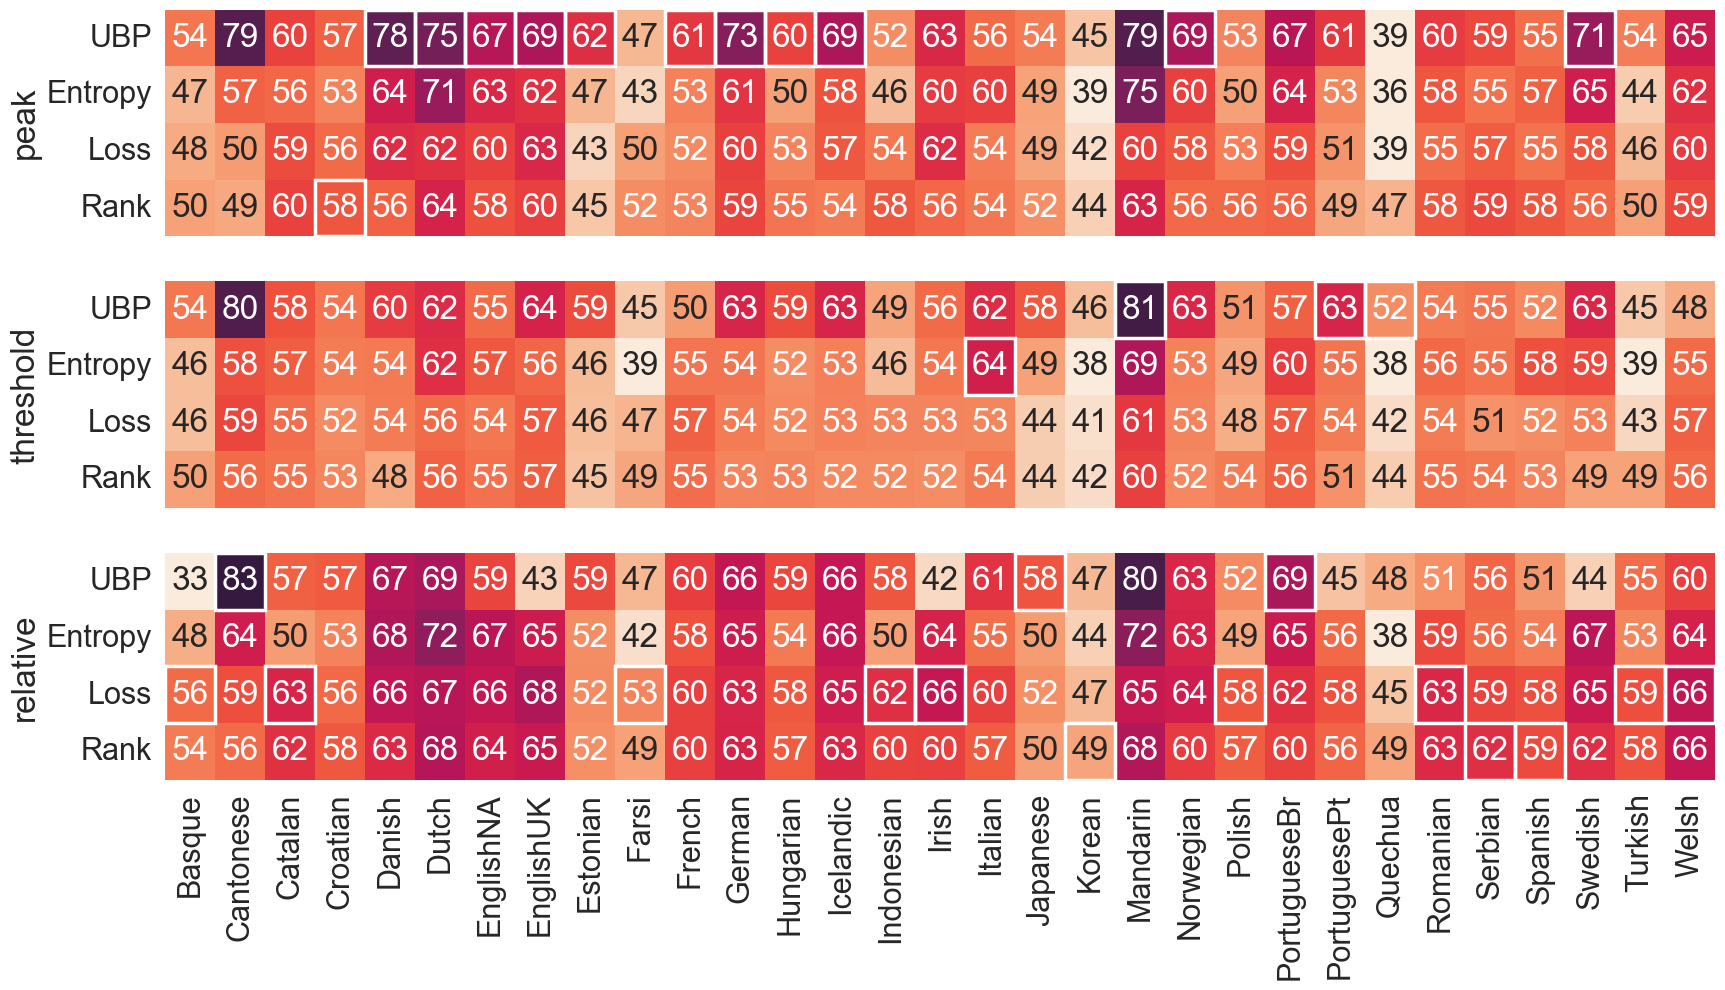
\includegraphics[width=0.99\linewidth]{Figures/15Phonology/tiny.png}
    \caption{Boundary placement F1 scores achieved by the models in the \textbf{Tiny} suite for each cue and segmentation strategy, with the highest score for each language highlighted.}
    \label{fig:15-tiny}
\end{figure}

\begin{figure}
    \centering
    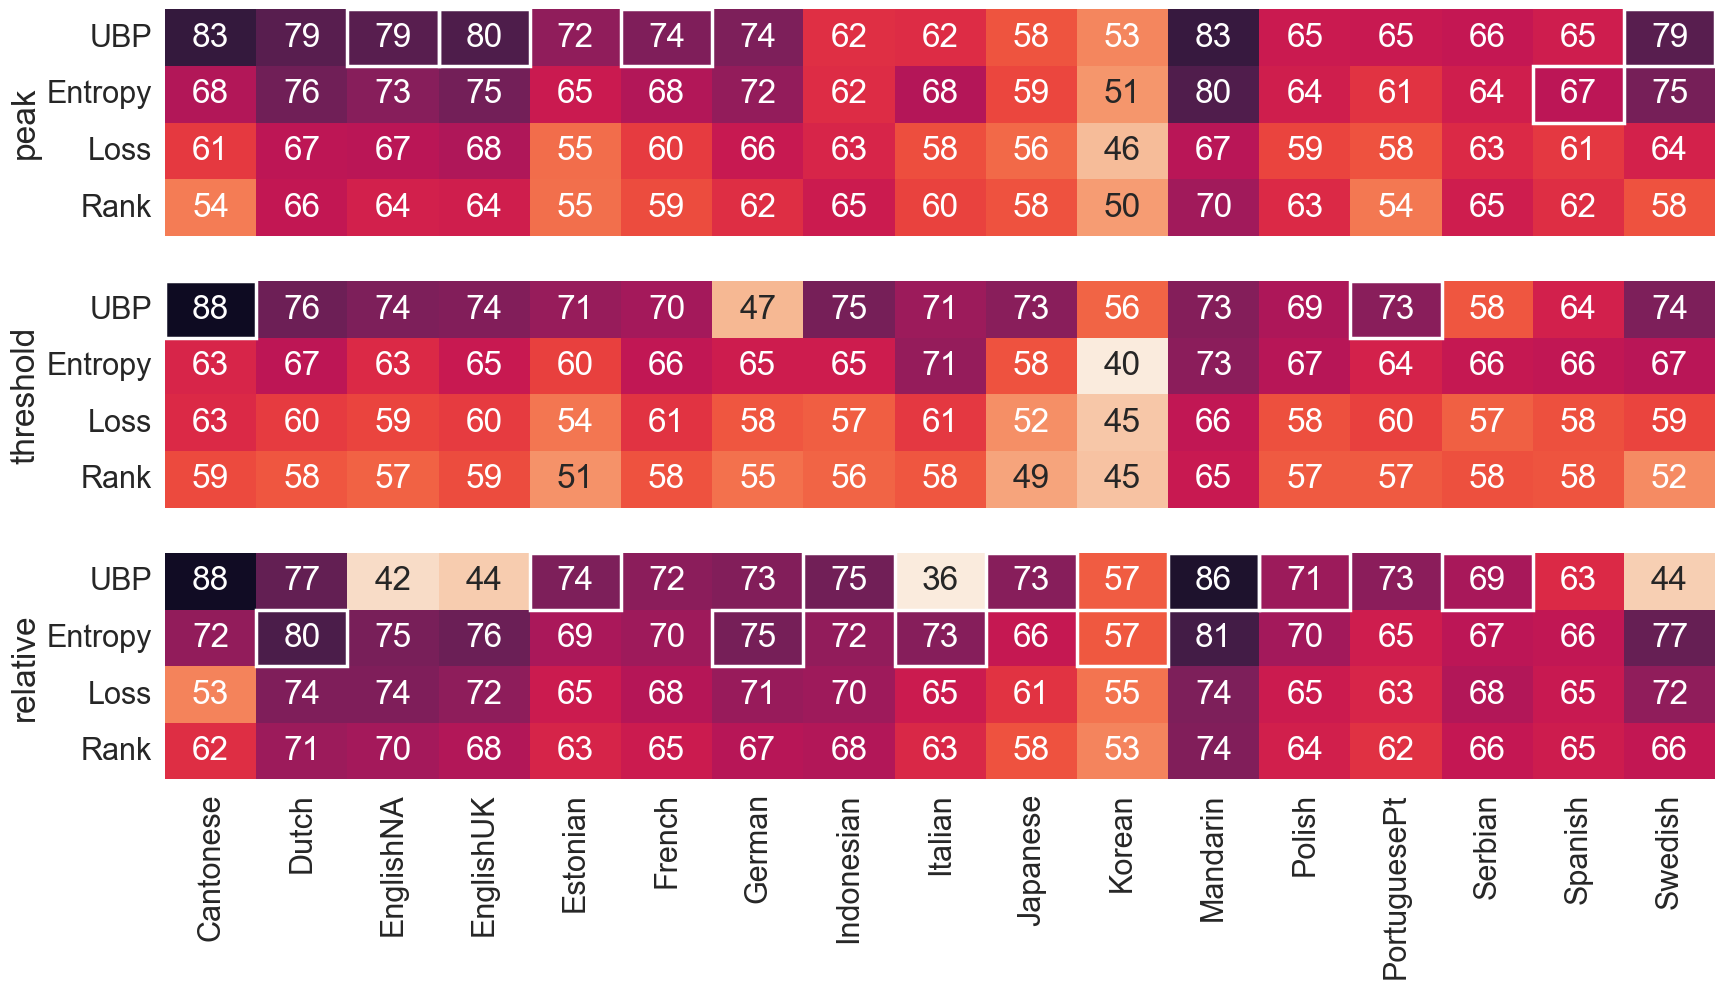
\includegraphics[width=0.99\linewidth]{Figures/15Phonology/small.png}
    \caption{Boundary placement F1 scores achieved by the models in the \textbf{Small} suite for each cue and segmentation strategy, with the highest score for each language highlighted.}
    \label{fig:15-small}
\end{figure}

\begin{figure}
    \centering
    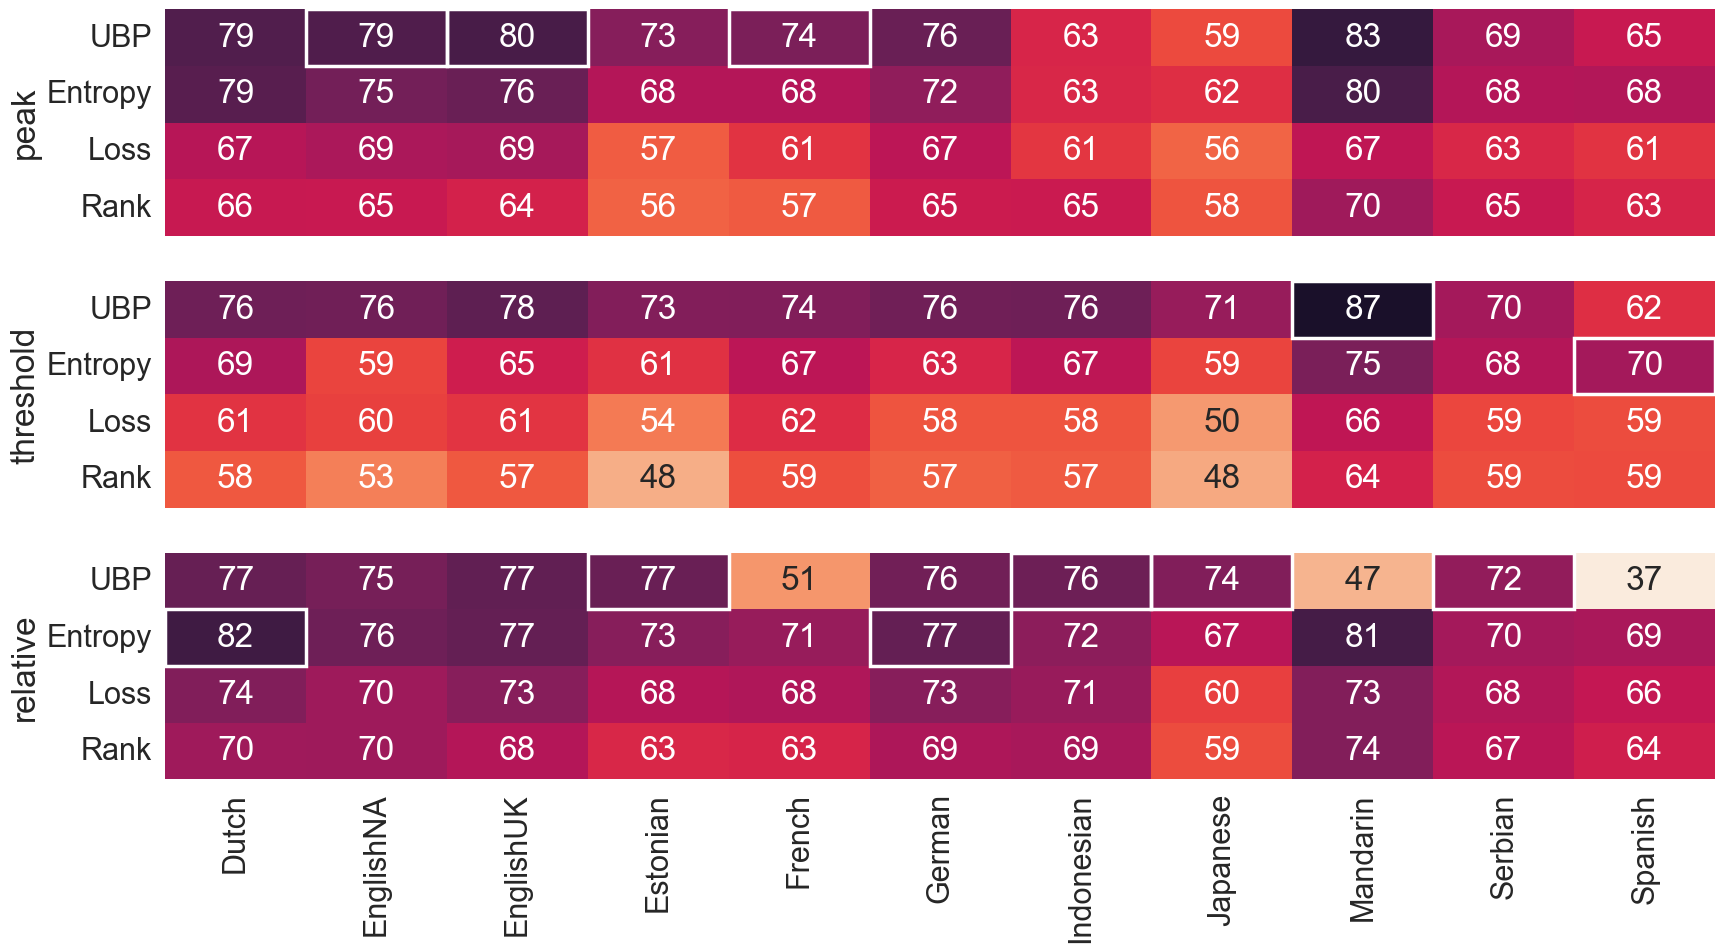
\includegraphics[width=0.99\linewidth]{Figures/15Phonology/medium.png}
    \caption{Boundary placement F1 scores achieved by the models in the \textbf{Medium} suite for each cue and segmentation strategy, with the highest score for each language highlighted.}
    \label{fig:15-medium}
\end{figure}

\begin{figure}
    \centering
    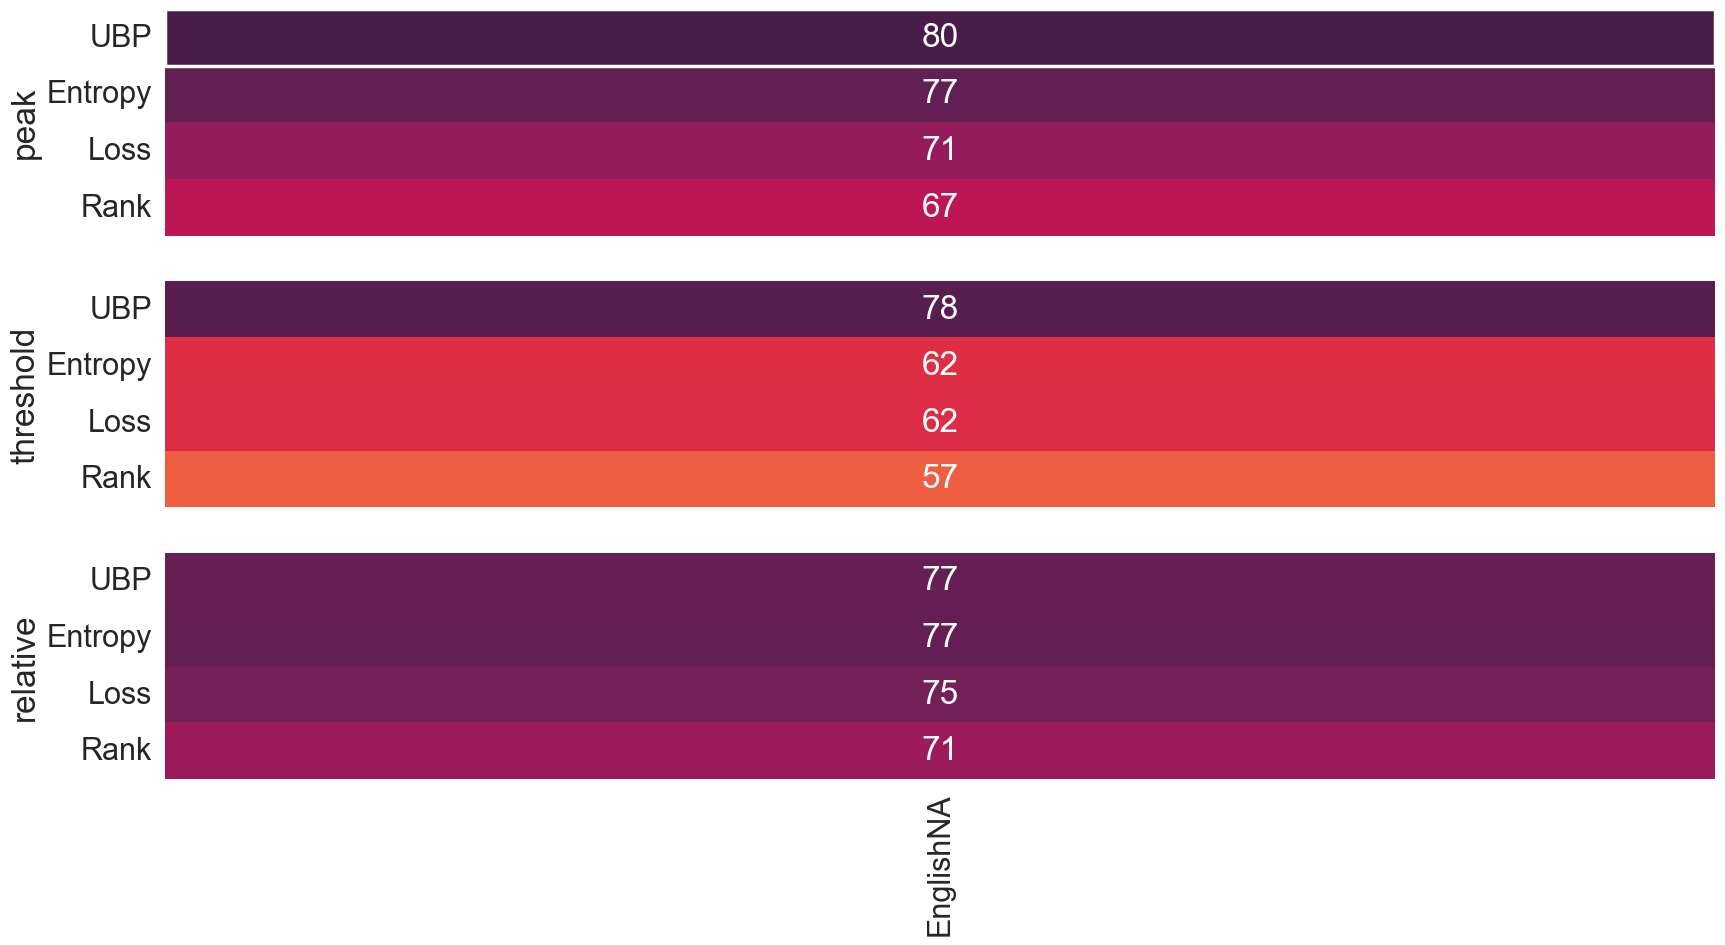
\includegraphics[width=0.99\linewidth]{Figures/15Phonology/large.png}
    \caption{Boundary placement F1 scores achieved by the models in the \textbf{Large} suite for each cue and segmentation strategy, with the highest score for each language highlighted.}
    \label{fig:15-large}
\end{figure}


\begin{table*}[t]
    \centering
    \footnotesize
    \begin{tabular}{lllll}
    \toprule
    Language & 100k & 700k & 2M & 18M \\
    \midrule
    Basque & Loss (relative) &  &  &  \\
    Cantonese & UBP (relative) & UBP (threshold) &  &  \\
    Catalan & Loss (relative) &  &  &  \\
    Croatian & Rank (peak) &  &  &  \\
    Danish & UBP (peak) &  &  &  \\
    Dutch & UBP (peak) & Entropy (relative) & Entropy (relative) &  \\
    EnglishNA & UBP (peak) & UBP (peak) & UBP (peak) & UBP (peak) \\
    EnglishUK & UBP (peak) & UBP (peak) & UBP (peak) &  \\
    Estonian & UBP (peak) & UBP (relative) & UBP (relative) &  \\
    Farsi & Loss (relative) &  &  &  \\
    French & UBP (peak) & UBP (peak) & UBP (peak) &  \\
    German & UBP (peak) & Entropy (relative) & Entropy (relative) &  \\
    Hungarian & UBP (peak) &  &  &  \\
    Icelandic & UBP (peak) &  &  &  \\
    Indonesian & Loss (relative) & UBP (relative) & UBP (relative) &  \\
    Irish & Loss (relative) &  &  &  \\
    Italian & Entropy (threshold) & Entropy (relative) &  &  \\
    Japanese & UBP (relative) & UBP (relative) & UBP (relative) &  \\
    Korean & Rank (relative) & Entropy (relative) &  &  \\
    Mandarin & UBP (threshold) & UBP (relative) & UBP (threshold) &  \\
    Norwegian & UBP (peak) &  &  &  \\
    Polish & Loss (relative) & UBP (relative) &  &  \\
    PortugueseBr & UBP (relative) &  &  &  \\
    PortuguesePt & UBP (threshold) & UBP (threshold) &  &  \\
    Quechua & UBP (threshold) &  &  &  \\
    Romanian & Loss (relative) &  &  &  \\
    Serbian & Rank (relative) & UBP (relative) & UBP (relative) &  \\
    Spanish & Rank (relative) & Entropy (peak) & Entropy (threshold) &  \\
    Swedish & UBP (peak) & UBP (peak) &  &  \\
    Turkish & Loss (relative) &  &  &  \\
    Welsh & Loss (relative) &  &  &  \\
    \bottomrule
    \end{tabular}
    \caption{Best combination of boundary cue and segmentation strategy for each language and each suite.}
    \label{tab:15-bestcuesfull}
\end{table*}
